\setdictum{%
  Beware of bugs in the above code;\\
  I have only proved it correct, not tried it.%
}{%
  Donald E.\ Knuth \cite{Knuth77Notes}%
}

\longchapter{%
  Application 2: Musculoskeletal Models%
}{%
  Application 2:\texorpdfstring{\\}{ }Musculoskeletal Models%
}{%
  Application 2 -- Musculoskeletal Models%
}
\label{chap:70muscle}

\initial{0em}{E}{xisting musculoskeletal models of muscle-tendon complexes,}
e.g., of the human upper limb, can mainly be divided into two different types.
\term{Lumped-parameter musculoskeletal models,}
for example Hill-type models based on multi-body simulations
\multicite{Roehrle16Two,Valentin18Gradient},
constitute the most common type.
These models assume that the components of the musculoskeletal system
are rigid.
The mechanics is reduced to point masses
associated with their moment of inertia;
thus, these models can be described by few parameters.

\term{Continuum-mechanical musculoskeletal models} form the other type.
Their advantage is that they are more detailed and, hence, more realistic.
However, their increased complexity leads to higher computational costs.
As an example, we consider an inverse problem (see \cref{chap:10introduction})
that involves a continuum-mechanical simulation of such a
musculoskeletal model,
where we search values of model parameters
such that a specific movement is attained.
Each iteration of the solution process for such an inverse problem
may take hours or even days, depending on the model at hand.

Surrogate methods based on sparse grids help to decrease the complexity
in two ways:
First, the evaluation of surrogates is obviously drastically cheaper
than the solution of the inverse problem.
Second, the particular choice of sparse grids decreases the number
of necessary samples to construct the surrogates.
As for the previous application,
the choice of B-splines as hierarchical basis functions enables
the evaluation of continuously differentiable surrogate gradients.
For the example of inverse problems, this means that
gradient-based optimization methods may be employed,
which significantly accelerates convergence compared to gradient-free methods.

This chapter is split into three sections.
First, in \cref{sec:71model}, we introduce a continuum-mechanical
model of the human upper limb.
Second, in \cref{sec:72methodology}, we list the types of inverse problems
of interest.
Finally, in \cref{sec:73results}, we present numerical results
regarding the solution of these inverse problems.

The results of this chapter are based on a collaboration with
Prof.\ Oliver Röhrle, PhD, and Dr.\ Michael Sprenger
(both SimTech/University of Stuttgart, Germany).%
\footnote{%
  Michael Sprenger left the University of Stuttgart in 2015.%
}
The collaborators contributed the biomechanical model
with its theory, its geometry, and its implementation,
while the author of this thesis contributed the
sparse grid/B-spline methodology and
computed the numerical results.
Note that the results have already been
published in a paper \cite{Valentin18Gradient},
which we will follow closely in this chapter.

\section{Continuum-Mechanical Model of the Upper Limb}
\label{sec:71model}

\minitoc{71mm}{6}

\noindent
In the following, we first discuss the state of the art
in biomechanical modeling.
Then, we address details of the model of the human upper limb.
For convenience, the most relevant symbols are listed in
\cref{tbl:glossaryMusculoskeletal}.

\begin{table}
  \setnumberoftableheaderrows{0}%
  \newcommand*{\pnst}[1]{%
    \printnotationsymbol{#1}%
    \vphantom{\printnotationsymbol{\equielbang}$(\cdot)^{\reference}$}&%
    \printnotationtext{#1}%
  }%
  \begin{tabular}{%
      >{\kern\tabcolsep}=l+l<{\kern5mm}+l+l<{\kern5mm}+l+l<{\kern\tabcolsep}%
    }
    \toprulec
    \pnst{\forceT}& \pnst{\armT}&       \pnst{\actT}\\
    \pnst{\forceB}& \pnst{\armB}&       \pnst{\actB}\\
    \pnst{\forceL}& \pnst{\armL}&       \pnst{\moment}\\
    \pnst{\elbang}& \pnst{\tarelbang}&  \pnst{\equielbang}\\
    \pnst{t}&
    $(\cdot)^{\sparse}$&Sparse grid solution&
    $(\cdot)^{\reference}$&Reference solution\\
    \bottomrulec
  \end{tabular}%
  \caption[Glossary for musculoskeletal models]{%
    Glossary of the notation for musculoskeletal models.%
  }%
  \label{tbl:glossaryMusculoskeletal}%
\end{table}



\subsection{Continuum-Mechanical Musculoskeletal Models}
\label{sec:711models}

\paragraph{%
  Limitations of classical models and
  benefits of continuum-mechanical models%
}

Due to the simplicity of classical lumped-parameter models,
their degree of realism is limited.
Without any modifications,
lumped-parameter models are not able to represent
detailed heterogeneous material characteristics or non-trivial
muscle force paths \cite{Roehrle16Two}.

The exploitation of continuum-mechani\-cal constitutive laws
for musculoskeletal models is a more recent development \cite{Roehrle16Two}.
The resulting models are capable to model spatial quantities
such as complex muscle fiber field architectures,
local activation principles, complex muscle geometries, or contact mechanics
\multicite{Roehrle16Two,Valentin18Gradient}.
Most of the existing work only treats single skeletal muscles in isolation
\multicite{Lemos05Modeling,Sharafi11Strains,Heidlauf14Multiscale}.
The model used in this thesis
(which is the same model as in
\multicite{Sprenger15Continuum,Roehrle16Two,Valentin18Gradient})
aims at studying the interplay of multiple muscles and bones.

\paragraph{Overdetermined antagonistic systems}

Musculoskeletal systems are typically overdetermined \cite{Roehrle16Two}.
This means that the number of muscles that act on a specific joint
is usually larger than the number of the joint's degrees of freedom.
For instance, in a simple model of the human upper limb,
there are two antagonistic muscles
(i.e., muscles that work against each other), namely triceps and biceps,
but only one joint angle at the elbow.
Mathematically speaking, a single muscle suffices to attain
a large range of elbow angles
that are possible with an antagonistic muscle pair.
However, the usage of two muscles enables faster movements and
allows for abrupt changes of direction.

The overdetermination of most musculoskeletal models
implies that additional conditions have to be imposed in order
to obtain unique solutions.
There exist various types of such conditions,
for instance, minimal control effort, minimal control change, and
minimal kinematic energy \cite{Valentin18Gradient}.
The idea behind these conditions is that the human body
tries to minimize the energy effort that is associated with
all types of motion.

\paragraph{Forward and inverse dynamics}

Musculoskeletal simulations are usually based on
either forward dynamics or inverse dynamics \cite{Valentin18Gradient}.
\term{Forward-dynamic approaches} use activation parameters
for the muscles as the input and simulate the corresponding motion
as the output.
This requires that we know the muscle forces
(depending on the activation levels) beforehand.
For example, one can prescribe activation levels of facial muscles
to achieve specific facial expressions \cite{Wu13Modelling}.
In contrast, \term{inverse-dynamic approaches}
use experimental motion data as the input
to estimate the muscle forces as the output \cite{Roehrle16Two}.
With inverse-dynamic simulations,
one can investigate the wrapping of muscles
around the knee joint \cite{Fernandez05Anatomically} or
visualize the motion of skin \cite{Lee09Comprehensive}, for instance.



\subsection{Details of the Human Upper Limb Model}
\label{sec:712details}

As shown in \cref{fig:raisingArm},
our model of the human upper limb consists
of the three bones humerus, ulna, and radius,
the elbow joint with one degree of freedom, and
the antagonistic muscle pair of triceps brachii and biceps brachii
\cite{Valentin18Gradient}.
The bones are rigid bodies and the muscle-tendon complex
is simulated with a continuum-mechanical approach.
This implies that the muscles deform when they contract.

\begin{figure}
  \begin{tikzpicture}[
    dashed/.style={dash pattern=on 2pt off 2pt},
    contour/.style={line width=3pt,draw=mittelblau!10},
  ]
    \newcommand*{\myhspace}{30.34mm}
    \newcommand*{\myscale}{0.14}
    \newcommand*{\mytricepsarmstart}{0.1}
    \newcommand*{\mybicepsstart}{0.2}
    \newcommand*{\myradius}{9mm}
    \newcommand*{\mysmallradius}{2mm}
    
    \foreach \myi in {1,...,5} {
      \node[anchor=north west] at ({(\myi-1)*\myhspace},0mm) {%
        \includegraphics[scale=\myscale]{upperLimb_\myi}%
      };
      \node[anchor=north west] at ({(\myi-1)*\myhspace+11mm},0mm) {%
        \pgfmathparse{10+35*(\myi-1)}%
        $\theta = \ang[
          round-mode=places,round-precision=0,
        ]{\pgfmathresult}$%
      };
    }
    
    \begin{scope}[shift={({(3-1)*\myhspace},0mm)}]
      \coordinate (joint)               at (8mm,-30mm);
      \coordinate (loadForceStart)      at (30.6mm,-35mm);
      \coordinate (loadForceEnd)        at (30.6mm,-45mm);
      \coordinate (tricepsForceStart)   at (5.7mm,-31.9mm);
      \coordinate (tricepsForceEnd)     at (4mm,-15mm);
      \coordinate (tricepsArmStart)     at (
        ${(1-\mytricepsarmstart)}*(joint) +
        \mytricepsarmstart*(loadForceStart)$
      );
      \coordinate (bicepsForceStart)    at (
        ${(1-\mybicepsstart)}*(joint) + \mybicepsstart*(loadForceStart)$
      );
      \coordinate (bicepsForceEnd)      at (11.5mm,-10mm);
      \coordinate (horizontalDashedEnd) at ($(loadForceEnd) + (0mm,3mm)$);
      \coordinate (verticalDashedEnd)   at ($(joint) - (0mm,15mm)$);
      \pgfmathanglebetweenpoints{
        \pgfpointanchor{joint}{center}
      }{
        \pgfpointanchor{loadForceStart}{center}
      }
      \let\myelbowangle\pgfmathresult
      \coordinate (arcStart) at ($(joint) - (0mm,\myradius)$);
      \coordinate (arcEnd) at (
        $(joint) + (
          {\myradius*cos(\myelbowangle)},
          {\myradius*sin(\myelbowangle)}
        )$
      );
      
      \makeatletter
      \newcommand*{\drawleverarm}[5][\@nil]{
        \def\myoptarg{#1}
        \ifx\myoptarg\@nnil
          \def\mypointsize{1pt}
          \def\myfill{C1}
          \def\myoptarg{}
        \else
          \def\mypointsize{2pt}
          \def\myfill{mittelblau!10}
        \fi
        \coordinate (leverArmBase) at ($(#3)!(#2)!(#4)$);
        \draw[dashed,draw=C1,\myoptarg] (#2) -- (leverArmBase);
        \pgfmathanglebetweenpoints{
          \pgfpointanchor{#2}{center}
        }{
          \pgfpointanchor{leverArmBase}{center}
        }
        \let\myangle\pgfmathresult
        \pgfmathparse{\myangle #5 180}
        \let\mystartangle\pgfmathresult
        \pgfmathparse{\myangle #5 90}
        \let\myendangle\pgfmathresult
        \centerarc[draw=C1,\myoptarg](leverArmBase)(
          \mystartangle:\myendangle:\mysmallradius
        );
        \fill[draw=none,fill=\myfill] (
          $(leverArmBase) + (
            {0.62*\mysmallradius*cos((\mystartangle+\myendangle)/2)},
            {0.62*\mysmallradius*sin((\mystartangle+\myendangle)/2)}
          )$
        ) circle (\mypointsize);
      }
      \makeatother
      
      \draw[contour] (joint) -- (loadForceStart);
      \draw[contour] (tricepsArmStart) -- (tricepsForceStart);
      
      \draw[dashed,contour] (joint) -- (verticalDashedEnd);
      \draw[dashed,contour] (
        $(joint)!(horizontalDashedEnd)!(verticalDashedEnd)$
      ) -- (horizontalDashedEnd);
      \draw[dashed,contour] (joint) -- (
        $(tricepsForceStart)!(joint)!(tricepsForceEnd)$
      );
      \draw[dashed,contour] (joint) -- (
        $(bicepsForceStart)!(joint)!(bicepsForceEnd)$
      );
      \centerarc[dashed,contour](joint)(270:\myelbowangle:\myradius);
      
      \drawleverarm[contour]{horizontalDashedEnd}{joint}{verticalDashedEnd}{-}
      \drawleverarm[contour]{joint}{tricepsForceStart}{tricepsForceEnd}{-}
      \drawleverarm[contour]{joint}{bicepsForceStart}{bicepsForceEnd}{+}
      
      \draw[
        ->,contour,>={Stealth[width=9pt,length=9pt]},
      ] (tricepsForceStart) -- (
        $(tricepsForceEnd)!-1.5pt!(tricepsForceStart)$
      );
      \draw[
        ->,contour,>={Stealth[width=9pt,length=9pt]},
      ] (bicepsForceStart) -- (
        $(bicepsForceEnd)!-1.5pt!(bicepsForceStart)$
      );
      \draw[
        ->,contour,>={Stealth[width=9pt,length=9pt]},
      ] (loadForceStart) -- (
        $(loadForceEnd)!-1.5pt!(loadForceStart)$
      );
      
      \draw (joint) -- (loadForceStart);
      \draw (tricepsArmStart) -- (tricepsForceStart);
      
      \draw[dashed] (joint) -- (verticalDashedEnd);
      \centerarc[dashed](joint)(270:\myelbowangle:\myradius);
      
      \drawleverarm{horizontalDashedEnd}{joint}{verticalDashedEnd}{-}
      \drawleverarm{joint}{tricepsForceStart}{tricepsForceEnd}{-}
      \drawleverarm{joint}{bicepsForceStart}{bicepsForceEnd}{+}
      
      \draw[->,draw=C0] (tricepsForceStart) -- (tricepsForceEnd);
      \draw[->,draw=C0] (bicepsForceStart) -- (bicepsForceEnd);
      \draw[->,draw=C0] (loadForceStart) -- (loadForceEnd);
      
      \fill[draw=none,fill=black] (joint) circle (2pt);
      
      \node at (
        $(joint) + (
          {0.62*\myradius*cos((270+\myelbowangle)/2)},
          {0.62*\myradius*sin((270+\myelbowangle)/2)}
        )$
      ) {\contour{mittelblau!10}{$\elbang$}};
      
      \node[anchor=south] at (
        $0.5*(joint) +
        0.5*(tricepsForceStart)!(joint)!(tricepsForceEnd) +
        (-1mm,1mm)$
      ) {\contour{mittelblau!10}{\textcolor{C1}{$\armT$}}};
      \node[anchor=south] at (
        $0.5*(joint) +
        0.5*(bicepsForceStart)!(joint)!(bicepsForceEnd) +
        (1mm,1mm)$
      ) {\contour{mittelblau!10}{\textcolor{C1}{$\armB$}}};
      \node[anchor=north] at (
        $0.5*(horizontalDashedEnd) +
        0.5*(joint)!(horizontalDashedEnd)!(verticalDashedEnd) +
        (0mm,-1mm)$
      ) {\contour{mittelblau!10}{\textcolor{C1}{$\armL$}}};
      
      \node[anchor=east] at (
        $0.2*(tricepsForceStart) + 0.8*(tricepsForceEnd) + (-1mm,0mm)$
      ) {\contour{mittelblau!10}{\textcolor{C0}{$\forceT$}}};
      \node[anchor=west] at (
        $0.2*(bicepsForceStart) + 0.8*(bicepsForceEnd) + (1mm,0mm)$
      ) {\contour{mittelblau!10}{\textcolor{C0}{$\forceB$}}};
      \node[anchor=west] at (
        $0.2*(loadForceStart) + 0.8*(loadForceEnd) + (1mm,0mm)$
      ) {\contour{mittelblau!10}{\textcolor{C0}{$\forceL$}}};
    \end{scope}
  \end{tikzpicture}%
  \caption[Human upper limb model geometry as a raising arm movement]{%
    Human upper limb model geometry shown as a raising arm movement
    for the elbow angles
    $\theta = \ang{10}$, \ang{45}, \ang{80},
    \ang{115}, and \ang{150} \emph{(from left to right).}
    For $\theta = \ang{80}$,
    the contributing forces \emph{\textcolor{C0}{(blue)}} and
    lever arms \emph{\textcolor{C1}{(red)}} are shown.
    Taken and adapted from
    \multicite{Sprenger15Continuum,Valentin18Gradient}.%
  }%
  \label{fig:raisingArm}%
\end{figure}

\paragraph{Overall stress components}

The continuum-mechanical part of the model
is based on the theory of finite elasticity.
When muscles deform, forces act on each infinitesimally small element
of the muscles, which is known as \term{stress.}
Usually, especially in linear elasticity,
stress is measured with the \term{Cauchy stress tensor}
(also called the \term{true stress}) \cite{Soennerlind13Why}.
For non-linear stress-strain relations,
one may use other measures such as the
\term{second Piola--Kirchhoff stress}.
The second Piola--Kirchhoff stress has the additional advantage
that it is defined along the material directions,
in contrast to the Cauchy stress tensor,
which measures the stress in coordinate directions \cite{Soennerlind13Why}.

In \multicite{Sprenger15Continuum,Roehrle16Two,Valentin18Gradient},
the strain energy function is defined such that the
resulting overall second Piola--Kirchhoff stress $\mat{S}_\mathrm{MTC}$ of
the muscle-tendon complex satisfies
\begin{equation}
  \mat{S}_\mathrm{MTC}
  = \mat{S}_\mathrm{iso} + \mat{S}_\mathrm{aniso} - p \mat{C}^{-1},
\end{equation}
where $\mat{S}_\mathrm{iso}$ and $\mat{S}_\mathrm{aniso}$
are the \term{isotropic and anisotropic parts} of the stress, respectively,
$p$ is the \term{hydrostatic pressure} to ensure incompressibility,
and $\mat{C}$ is the \term{right Cauchy--Green deformation tensor.}
The anisotropic part $\mat{S}_\mathrm{aniso}$ is defined as
\begin{equation}
  \mat{S}_\mathrm{aniso}
  \ceq (
    \mat{S}_\mathrm{passive} +
    \act \gamma_\mathrm{M} \mat{S}_\mathrm{active}
  ) (1 - \gamma_\mathrm{ST}),
\end{equation}
cf.\ \cite{Valentin18Gradient}.
Here, $\mat{S}_\mathrm{passive}$ and $\mat{S}_\mathrm{active}$
are the \term{passive and active contributions}
due to the skeletal muscle fibers,
$\act \in \clint{0, 1}$ is the \term{activation parameter} of the
respective muscle-tendon complex, and
$\gamma_\mathrm{M}, \gamma_\mathrm{ST}$ are two \term{material parameters}
with which we can differentiate between the different types of soft tissues
of the muscle-tendon complex: fat, tendon, and muscle
\cite{Valentin18Gradient}.
Isotropic fat tissue can be obtained
by setting $\gamma_\mathrm{ST} \ceq 1$,
passive anisotropic tendon tissue
by setting $\gamma_\mathrm{ST} \ceq 0$ and $\gamma_\mathrm{M} \ceq 0$, and
skeletal muscle tissue
by setting $\gamma_\mathrm{ST} \ceq 0$ and $\gamma_\mathrm{M} \ceq 1$.
A mixture of these pure materials is
achieved by linear interpolation when setting
$\gamma_\mathrm{M}$ and $\gamma_\mathrm{ST}$ to values between zero and one
\cite{Valentin18Gradient}.
More details about the theory part of the model are given in
\multicite{Sprenger15Continuum,Roehrle16Two,Valentin18Gradient}.

\section{Momentum Equilibrium and Elbow Angle Optimization}
\label{sec:72methodology}

\minitoc[-7mm]{70mm}{4}

\noindent
In this section, we give an overview of the methodology of our approach.
We continue following the presentation of \cite{Valentin18Gradient}.



\subsection{From Muscle Forces to Equilibrium Angles}
\label{sec:721equilibrium}

\paragraph{Model inputs and outputs}

In the following, we regard simulations of the
human upper limb model described in \cref{sec:71model} as a black box,
which receives as its input
the elbow angle $\elbang \in \clint{\ang{10}, \ang{150}}$
and the activation parameters
$(\actT, \actB) \in \clint{\*0, \*1} = \clint{0, 1}^2$
of triceps and biceps.%
\footnote{%
  Here and in the following, the subscripts T, B, and L stand for
  triceps, biceps, and load, respectively.%
}
The outputs of the black box simulation are the forces
$\forceT(\elbang, \actT)$ and $\forceB(\elbang, \actB)$
that triceps and biceps exert.
These forces depend on the elbow angle as well as on the respective
activation parameter.
Gravitational forces due to the masses of bones or muscles
are neglected in this context.
However, we allow the specification of an external load $\forceL$,
which is applied to the end of the forearm.
This load may be the weight force of some object
that the arm is supposed to keep in position.

\paragraph{Moments and lever arms}

Each force exerts a \term{moment} (or \term{torque}) on the elbow joint.
The moments are the products of the forces $\forceX$
with the respective lever arms $\armX$
($X \in \{\mathrm{T}, \mathrm{B}, \mathrm{L}\}$).
The lever arms are approximated as in
\multicite{Roehrle16Two,Valentin18Gradient} by using
the tendon-displacement method of \cite{An84Determination}:
\begin{subequations}
  \begin{align}
    \armT(\elbang)
    &\ceq (-0.0009399 \{\elbang\}^2 + 0.1126 \{\elbang\} + 22.21)\;
    \si{\milli\meter},\\
    \armB(\elbang)
    &\ceq (-0.001482 \{\elbang\}^2 + 0.1776 \{\elbang\} + 35.02)\;
    \si{\milli\meter},\\
    \armL(\elbang)
    &\ceq \sin(\elbang) \cdot \SI{282.5}{\milli\meter},
  \end{align}
\end{subequations}
where $\{\elbang\}$ denotes the dimensionless value of $\elbang$
in degrees.
The lever arms are non-negative and the forces are signed, i.e.,
positive forces pull the forearm downwards and
negative forces pull it upwards.
In general, $\forceT, \forceL \ge \SI{0}{\newton}$ and
$\forceB \le \SI{0}{\newton}$.

\paragraph{Total moment and equilibrium elbow angle}

The \term{total moment} of the system is given by the function
\begin{subequations}
  \label{eq:totalMoment}
  \begin{gather}
    \moment_{\forceL,\actT,\actB}\colon
    \clint{\ang{10}, \ang{150}} \to \real,\\
    \moment_{\forceL,\actT,\actB}(\elbang)
    \ceq \forceT(\elbang, \actT) \armT(\elbang) +
    \forceB(\elbang, \actB) \armB(\elbang) +
    \forceL \armL(\elbang),
  \end{gather}
\end{subequations}
cf.\ \cite{Valentin18Gradient}.
The system is in \term{equilibrium}
if the total moment vanishes, i.e.,
$\moment_{\forceL,\actT,\actB}(\elbang) = \SI{0}{\newton\meter}$.
We call the corresponding angle $\elbang$ the
\term{equilibrium elbow angle}
for the load $\forceL$ and the activation parameters $\actT, \actB$.
To find this angle for a given load $\forceL$ and activation parameters
$\actT$ and $\actB$, we first note that
$\moment_{\forceL,\actT,\actB}$ may have zero, exactly one,
or multiple zeros in $\clint{\ang{10}, \ang{150}}$.
Hence, the inverse function evaluated at $\SI{0}{\newton\meter}$
is partially defined depending on the load and the activation parameters:
\begin{equation}
  \label{eq:equilibriumAngle}
  \equielbang{\forceL}\colon \actdomain{\forceL} \!\to
  \clint{\ang{10}, \ang{150}},\quad
  \actdomain{\forceL} \subset \clint{\*0, \*1},\quad
  \equielbang{\forceL}(\actT,\actB)
  \ceq (\moment_{\forceL,\actT,\actB})^{-1}(\SI{0}{\newton\meter}),
\end{equation}
which is well-defined whenever $\moment_{\forceL,\actT,\actB}$
has a unique root.
We approximate $\equielbang{\forceL}(\actT,\actB)$ with the Newton method
\multicite{Roehrle16Two,Valentin18Gradient}:
\begin{equation}
  \label{eq:newtonAngle}
  \elbang^{(j+1)}
  \ceq \elbang^{(j)} -
  \frac{
    \moment_{\forceL,\actT,\actB}(\elbang^{(j)})
  }{
    \partialderiv{\partialdiff{} \elbang}{\moment_{\forceL,\actT,\actB}}
    (\elbang^{(j)})
  },\quad
  j \in \nat,
\end{equation}
with an initial value
$\elbang^{(0)} \in \clint{\ang{10}, \ang{150}}$
and the stopping criterion of
$\abs{\moment_{\forceL,\actT,\actB}(\elbang^{(j)})} <
\SI{e-9}{\newton\meter}$.
We repeat the Newton method for the initial values
$\elbang^{(0)} = \ang{80}, \ang{40}, \ang{120}$
and use the first converged result
(i.e., we check if $\elbang^{(0)} = \ang{80}$ converges;
if not, we proceed with $\elbang^{(0)} = \ang{40}$, and so on).
If all three initial values do not converge,
we conclude that $(\actT, \actB) \notin \actdomain{\forceL}$.



\subsection{Optimization Problems}
\label{sec:722optimization}

\paragraph{General problem}

The general problem in our setting is as follows:
For a given external load $\forceL$ and a target elbow angle $\tarelbang$,
find activation parameters $(\actT, \actB) \in \clint{\*0, \*1}$
such that the target elbow angle is attained in the equilibrium,
i.e., $\equielbang{\forceL}(\actT,\actB) = \tarelbang$.
Example applications of such a scenario are medicine and robotics,
when a specific movement should be carried out.

\paragraph{List of optimization problems}

As discussed in \cref{sec:711models},
musculoskeletal systems with an antagonistic muscle pair
such as our human upper limb model are usually overdetermined.
This means that there are multiple solutions to this general problem.
As a remedy, one may solve one of the following two
optimization problems \cite{Valentin18Gradient}:

\begin{enumerate}[label=O\arabic*.,ref=O\arabic*,leftmargin=2.7em]
  \item
  \label{item:biomech2MinSum}
  For a given external load $\forceL$ and a target angle
  $\tarelbang \in \clint{\ang{10}, \ang{150}}$,
  find the activation parameters $(\actT, \actB) \in \clint{\*0, \*1}$
  such that $\actT + \actB$ is minimized under the constraint
  $\equielbang{\forceL}(\actT, \actB) = \tarelbang$.
  
  \item
  \label{item:biomech2MinDist}
  For a given external load $\forceL(t_2)$ for a time $t_2 > t_1$,
  a target angle $\tarelbang(t_2) \in \clint{\ang{10}, \ang{150}}$,
  and initial activation parameters
  $(\actT(t_1), \actB(t_1)) \in \clint{\*0, \*1}$,
  find new activation parameters
  $(\actT(t_2), \actB(t_2)) \in \clint{\*0, \*1}$ such that
  $(\actT(t_2) - \actT(t_1))^2 + (\actB(t_2) - \actB(t_1))^2$
  is minimized under the constraint
  $\equielbang{\forceL(t_2)}(\actT(t_2), \actB(t_2)) = \tarelbang(t_2)$.
\end{enumerate}

\noindent
The motivation of both problems is that the human body tries to
achieve a given movement with minimal energy effort.

\paragraph{Motivation of problem \ref{item:biomech2MinSum}}

For the first problem \ref{item:biomech2MinSum},
this effort is quantified by $\actT + \actB$,
i.e., the energy effort for each muscle is assumed to be proportional
to its activation parameter.

\paragraph{Motivation of problem \ref{item:biomech2MinDist}}

The second problem \ref{item:biomech2MinDist} is motivated as follows:
Before time $t = t_1$, the musculoskeletal system is in equilibrium for
the external load $\forceL(t_1)$,
activation parameters $\actT(t_1), \actB(t_1)$, and elbow angle
$\tarelbang(t_1) \ceq \equielbang{\forceL(t_1)}(\actT(t_1), \actB(t_1))$, i.e.,
$\moment_{\forceL(t_1),\actT(t_1),\actB(t_1)}(\tarelbang(t_1))
= \SI{0}{\newton\meter}$.
Directly after $t = t_1$,
the external force and/or the target angle is suddenly changed
to $\forceL(t_2)$ and $\tarelbang(t_2)$, respectively.
Consequently, triceps and biceps adapt their activation parameters
such that the musculoskeletal system returns to equilibrium
at some time $t = t_2 > t_1$.
Hence, we have to determine the new activation parameters
$\actT(t_2), \actB(t_2)$ such that
$\moment_{\forceL(t_2),\actT(t_2),\actB(t_2)}(\tarelbang(t_2))
= \SI{0}{\newton\meter}$.
Again, these parameters
$\actT(t_2)$ and $\actB(t_2)$ are not uniquely determined.
Therefore, we want to find the pair of activation parameters
that is closest (in terms of the Euclidean norm) to the initial
activation parameters $\actT(t_1), \actB(t_1)$.

\paragraph{Optimization method}

Problems \ref{item:biomech2MinSum} and \ref{item:biomech2MinDist}
are both constrained optimization problems.
For their solution, we employ the augmented Lagrangian method as
described in \cref{sec:513gradientBasedConstrained}
using an adaptive gradient descent algorithm
for the gradient-based optimization of the penalized objective function
(see \cref{sec:512gradientBasedUnconstrained}).



\subsection{B-Spline Surrogates on Sparse Grids}
\label{sec:723surrogates}

\paragraph{Complexity}

To solve optimization problems
\ref{item:biomech2MinSum} and \ref{item:biomech2MinDist},
the optimization method needs to evaluate the objective
and constraint functions multiple times during the algorithm.
This requires the evaluation of $\equielbang{\forceL}$,
which in turn has to be approximated with the Newton method.
As we see in \cref{eq:newtonAngle},
each iteration of the Newton method needs not only the values of the
muscle forces $\forceT$ and $\forceB$, but also their
partial derivatives with respect to $\elbang$.
These partial derivatives have to be approximated with finite differences.

Unfortunately, simulations of continuum-mechanical models are
computationally expensive.
One evaluation of the muscle force pair $\forceT, \forceB$
requires the solution of a solid mechanics model
with a complex constitutive law, pre-stretch, and contact between
bone and muscles \cite{Valentin18Gradient}.
On average, a single evaluation of $\forceT$ and $\forceB$ takes
about half an hour on current desktop computers.
%
If we assume that we need four Newton iterations on average,
then a single iteration of the optimization algorithm to solve
problems \ref{item:biomech2MinSum} and \ref{item:biomech2MinDist}
will take four hours to complete
(assuming one evaluation of objective and constraint functions
per optimizer iteration and
two evaluations of the muscle force pair
per Newton iteration to approximate the missing derivative).
Consequently, the whole optimization process takes
two weeks to complete, if the optimizer converges after 100 iterations.

\paragraph{Sparse grid surrogates}

A popular way to reduce complexity is to employ surrogates.
In this case, the idea is to replace the muscle force functions
$\forceT, \forceB$ with surrogates $\forceTintp, \forceBintp$
\cite{Valentin18Gradient}, e.g., by interpolation.
We then automatically obtain a surrogate
\begin{subequations}
  \label{eq:totalMomentSurrogate}
  \begin{gather}
    \momentintp_{\forceL,\actT,\actB}\colon
    \clint{\ang{10}, \ang{150}} \to \real,\\
    \momentintp_{\forceL,\actT,\actB}(\elbang)
    \ceq \forceTintp(\elbang, \actT) \armT(\elbang) +
    \forceBintp(\elbang, \actB) \armB(\elbang) +
    \forceL \armL(\elbang),
  \end{gather}
\end{subequations}
for the total moment (cf.\ \cref{eq:totalMoment}) and,
consequently, a surrogate
\begin{equation}
  \label{eq:equilibriumAngleSurrogate}
  \equielbangintp{\forceL}\colon \actdomainintp{\forceL} \!\to
  \clint{\ang{10}, \ang{150}},\quad
  \actdomainintp{\forceL} \subset \clint{\*0, \*1},\quad
  \equielbangintp{\forceL}(\actT,\actB)
  \ceq (\momentintp_{\forceL,\actT,\actB})^{-1}(\SI{0}{\newton\meter}),
\end{equation}
for the equilibrium elbow angle function (cf.\ \cref{eq:equilibriumAngle}).
Since the surrogates are much cheaper to evaluate,
the computation time is decreased by up to seven orders of magnitude,
as experiments show.

The approach in \cite{Valentin18Gradient} and in this thesis is
to determine surrogates
$\forceXintp\colon \clint{\*0, \*1} \to \real$
($X \in \{\mathrm{T}, \mathrm{B}\}$) by sparse grid interpolation.
Compared to surrogate construction techniques based on full grids,
sparse grids help to reduce the number of samples that
are necessary to build ``reasonably'' accurate surrogates,
especially if the number of dimensions is moderately large
($d \ge 4$, \term{curse of dimensionality}).

The present model only has $d = 2$ dimensions ($\actT$ and $\actB$),
since the model contains only two muscles.
However, as we will see,
already for this low-dimensional problem,
sparse grids outperform conventional full grid interpolation.
The results have to be seen as a proof of concept.
One will be able to handle higher dimensionalities
(i.e., models with a larger number of muscles) similarly with little
or even no adjustments at all.
The low dimensionality of the model in this thesis
enables us to compute and compare against reference solutions,
which would not be possible in a higher-dimensional setting.



\paragraph{Benefiting from B-splines}

As in \cite{Valentin18Gradient},
we use higher-order hierarchical B-splines as basis functions
for the sparse grid surrogates.
This has three advantages when compared with conventional
sparse grid bases such as piecewise linear functions:
%
First, the partial derivative
$\partialderiv{\partialdiff{} \elbang}{\momentintp}$ needed
for the Newton method in \cref{eq:newtonAngle} is continuous and
explicitly known.
There is no need to approximate the derivative with
finite differences, reducing both error and computation time.
%
Second, we can use gradient-based optimization methods
for the solution of the optimization problems \ref{item:biomech2MinSum} and
\ref{item:biomech2MinDist},
which involve the equilibrium elbow angle function
$\equielbangintp{\forceL}\colon \clint{\*0, \*1} \to \real$.
With the implicit function theorem \cite{Kudryavtsev95Implicit},
we obtain for the derivative of $\equielbangintp{\forceL}$
\begin{equation}
  \gradient{\actT,\actB}{\equielbangintp{\forceL}}
  = -\,(\gradient{\actT,\actB}{\momentintp}) \cdot
  (\gradient{\elbang}{\momentintp})^{-1}
  = -\,\frac{
    \gradient{\actT,\actB}{\momentintp}
  }{
    \partialderiv{\partialdiff{} \elbang}{\momentintp}
  },
\end{equation}
where $\gradient{\actT,\actB}{}$ is the transposed Jacobian
with respect to $\actT$ and $\actB$.%
\footnote{%
  For example, the first column is the gradient with respect to $\actT$
  and the second column is the gradient with respect to $\actB$.%
}
For B-splines,
both the transposed Jacobian $\gradient{\actT,\actB}{\momentintp}$ and
the partial derivative $\partialderiv{\partialdiff{} \elbang}{\momentintp}$
are continuous, explicitly known, and can be evaluated fast.
%
Third and finally,
the usage of higher-order B-splines as basis functions
increases the order of convergence of interpolation errors
as shown for test functions in \cref{sec:541interpolation}.
Thus, fewer interpolation points are necessary to construct a surrogate
with the same error as for piecewise linear functions.

\breakpagebeforenextheadingtrue
\section{Implementation and Numerical Results}
\label{sec:73results}

\minitoc[0mm]{69mm}{8}

\parbox{1em}{}
\vspace{-3em}



\disableornamentsfornextheadingtrue
\subsection{Implementation}
\label{sec:731implementation}

\paragraph{Parameters, implementation, and geometry}

Details about implementational aspects of the model can be found in
\multicite{Sprenger15Continuum,Roehrle16Two,Valentin18Gradient},
for instance, values for the material parameters.
%
The constitutive law has been implemented in the CMISS software package
(an interactive computer program for Continuum Mechanics,
Image analysis, Signal processing and System identification%
\footnote{%
  \url{https://www.cmiss.org/}%
}).
The emerging PDEs are discretized using quadratic finite element basis
functions and the resulting linearized system is solved with CMISS.
%
The geometry of the human upper limb model is based on
the Visible Human Male's dataset \cite{Spitzer96Visible}.
Again, we refer to \multicite{Sprenger15Continuum,Roehrle16Two} for details
about the geometry.



\subsection{Reference and Sparse Grid Solution}
\label{sec:732solutionTypes}

\paragraph{Reference solution}

Since the model is only two-dimensional, we can compute a reference solution
on a full grid.
To this end, we evaluate the exerted muscle forces $\forceT$ and $\forceB$ on
the full grid
\begin{equation}
  \{\ang{10}, \ang{11}, \dotsc, \ang{150}\} \times \{0, 0.1, \dotsc, 1\}
  \ni (\elbang, \actX),\quad
  X \in \{\mathrm{T}, \mathrm{B}\}.
\end{equation}
The resulting \num{1551} grid points
are interpolated with bicubic full grid splines%
\footnote{%
  Computed with the Geometric Tools Engine \cite{Schneider03Geometric},
  see \url{https://www.geometrictools.com/}.%
}
to obtain \term{reference solutions}
$\forceTref, \forceBref\colon
\clint{\ang{10}, \ang{150}} \times \clint{0, 1} \to \real$,
which are shown in \cref{fig:biomech2ReferenceForce}.
Due to the high resolution of the full grid,
we may assume that the reference solutions are accurate enough
to ensure $\forceTref \approx \forceT$ and $\forceBref \approx \forceB$.
We refer to the resulting equilibrium elbow angle
with $\equielbangref{\forceL}$.
It is displayed in
\cref{fig:biomech2ReferenceEquilibriumAngle}
for the loads of $\forceL = \SI{22}{\newton}$,
$\SI{-60}{\newton}$, and $\SI{180}{\newton}$.

\begin{figure}
  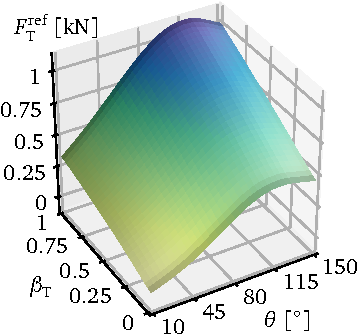
\includegraphics{biomech2ReferenceForce_1}%
  \;\;%
  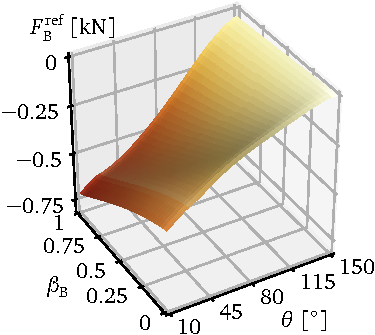
\includegraphics{biomech2ReferenceForce_2}%
  \hfill%
  \rlap{\raisebox{53mm}{\;$\forceXref$ [\si{\kilo\newton}]}}%
  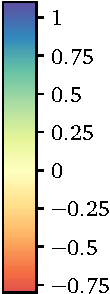
\includegraphics{biomech2ReferenceForce_3}%
  \caption[Reference triceps and biceps forces]{%
    Reference triceps and biceps forces $\forceXref$
    ($X \in \{\mathrm{T}, \mathrm{B}\}$).%
  }%
  \label{fig:biomech2ReferenceForce}%
\end{figure}

\begin{figure}
  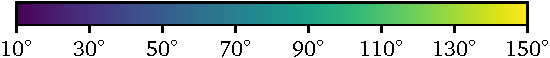
\includegraphics{biomech2ReferenceEquilibriumAngle_4}%
  \\[2mm]%
  \subcaptionbox{%
    $\forceL = \SI{22}{\newton}$%
  }[49mm]{%
    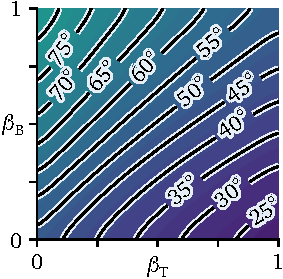
\includegraphics{biomech2ReferenceEquilibriumAngle_1}%
  }%
  \hfill%
  \subcaptionbox{%
    $\forceL = \SI{-60}{\newton}$%
  }[49mm]{%
    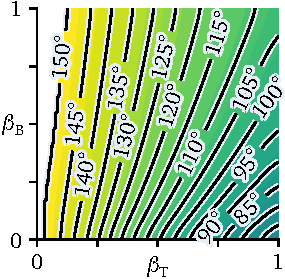
\includegraphics{biomech2ReferenceEquilibriumAngle_2}%
  }%
  \hfill%
  \subcaptionbox{%
    $\forceL = \SI{180}{\newton}$%
  }[49mm]{%
    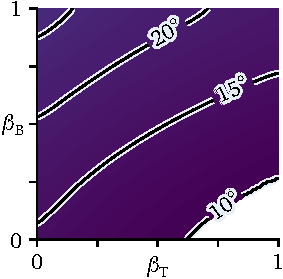
\includegraphics{biomech2ReferenceEquilibriumAngle_3}%
  }%
  \caption[Reference equilibrium elbow angle]{%
    Reference equilibrium elbow angle $\equielbangref{\forceL}$
    for different loads $\forceL$.
    The empty areas correspond to activation pairs
    at which $\equielbangref{\forceL}$ is not well-defined
    (see \cref{eq:equilibriumAngle}).%
  }%
  \label{fig:biomech2ReferenceEquilibriumAngle}%
\end{figure}

\paragraph{Sparse grid solution}

Additionally, we evaluate $\forceT$ and $\forceB$ at the $\ngp = 49$
grid points
\begin{equation}
  \{(\elbang^{(k,\mathrm{unif})}, \actX^{(k,\mathrm{unif})}) \mid
  k = 1, \dotsc, \ngp\}
  \subset \clint{\ang{10}, \ang{150}} \times \clint{0, 1},\quad
  X \in \{\mathrm{T}, \mathrm{B}\},
\end{equation}
of the uniform regular sparse grid $\interiorregsgset{n}{d}$ of
level $n = 5$ in $d = 2$ dimensions
without boundary points (to reduce the number of samples)
and at the sparse Clenshaw--Curtis grid
\begin{equation}
  \{(\elbang^{(k,\cc)}, \actX^{(k,\cc)}) \mid
  k = 1, \dotsc, \ngp\}
  \subset \clint{\ang{10}, \ang{150}} \times \clint{0, 1},\quad
  X \in \{\mathrm{T}, \mathrm{B}\},
\end{equation}
of the same size and level.%
\footnote{%
  The domain $\clint{\ang{10}, \ang{150}} \times \clint{0, 1}$
  is assumed to be implicitly normalized to the unit square
  $\clint{\*0, \*1}$.%
}
These values are interpolated using three
different hierarchical B-spline bases of degree $p = 1$, $3$, and $5$:
modified hierarchical uniform B-splines
$\bspl[\modified]{\*l,\*i}{p}$
(see \cref{sec:313modification}),
modified hierarchical Clenshaw--Curtis B-splines
$\bspl[\cc,\modified]{\*l,\*i}{p}$
(see \cref{sec:314nonUniform}), and
modified hierarchical uniform not-a-knot B-splines
$\bspl[\nak,\modified]{\*l,\*i}{p}$
(see \cref{sec:323modifiedNAKBSplines}).
The implementation was done using the sparse grid toolbox
\sgpp{} \cite{Pflueger10Spatially}.%
\footnote{%
  \url{http://sgpp.sparsegrids.org/}%
}
The corresponding interpolants and resulting quantities
are denoted with the superscripts
``$\sparse,\!p$'', ``$\sparse,\!p,\!\cc$'', or ``$\sparse,\!p,\!\nak$'',
respectively.
A superscript of ``$\sparse$'' without any further specification
means one of the three hierarchical B-spline bases in general.
Note that the equilibrium elbow angle is \emph{not} interpolated
(neither in the full grid nor in the sparse grid case),
but rather obtained by inserting the interpolated muscle forces
into \eqref{eq:totalMomentSurrogate} and \eqref{eq:equilibriumAngleSurrogate}.



\subsection{Errors of Muscle Forces and Equilibrium Angle}
\label{sec:733errors}

\paragraph{Quality of reference interpolants}

Before we turn to the sparse grid interpolants,
we assess the quality of the reference interpolants on the full grid.
For this purpose, we evaluate the full grid interpolants
$\forceTintp, \forceBintp$
at the sparse grid points $(\elbang^{(k)}, \actX^{(k)})$
(which are not a subset of the full grid points!)
and compare the resulting values with the known exact values
$\forceT(\elbang^{(k)}, \actT^{(k)})$ and
$\forceB(\elbang^{(k)}, \actB^{(k)})$
of the muscle forces $\forceT, \forceB$.
We also incorporate the known values at the sparse
Clenshaw--Curtis grid points.
In particular, let $G$ be the union of
$\{(\elbang^{(k,\mathrm{unif})}, \actX^{(k,\mathrm{unif})}) \mid
k = 1, \dotsc, \ngp\}$ and
$\{(\elbang^{(k,\cc)}, \actX^{(k,\cc)}) \mid k = 1, \dotsc, \ngp\}$.
We then approximate the relative $\Ltwo$ interpolation error
of the reference interpolants by
\begin{equation}
  \frac{\normLtwo{\forceX - \forceXref}}{\normLtwo{\forceX}}
  \approx
  \frac{
    \setsize{G}^{-1/2}
    \norm[2]{
      (\forceX(\elbang, \actX) - \forceXref(\elbang, \actX))_
      {(\elbang, \actX) \in G}
    }
  }{
    \setsize{G}^{-1/2}
    \norm[2]{(\forceX(\elbang, \actX))_{(\elbang, \actX) \in G}}
  },\quad
  X \in \{\mathrm{T}, \mathrm{B}\},
\end{equation}
where $\norm[2]{\cdot}$ is the Euclidean norm.%
\footnote{%
  We have $\setsize{G} = 2\ngp - 1$, since sparse grids of
  uniform and Clenshaw--Curtis type only
  share the center point $(\elbang, \actX) = (\ang{80}, 0.5)$,
  if there are no boundary points.%
}
After inserting the known values $\forceX(\elbang, \actX)$ and
$\forceXref(\elbang, \actX)$ ($(\elbang, \actX) \in G$)
on the right-hand side,
we obtain
\begin{equation}
  \frac{\normLtwo{\forceT - \forceTref}}{\normLtwo{\forceT}}
  \approx \SI{2.19}{\permille},\qquad
  \frac{\normLtwo{\forceB - \forceBref}}{\normLtwo{\forceB}}
  \approx \SI{2.06}{\permille}.
\end{equation}
These errors are very small, which justifies our assumption of
$\forceTref \approx \forceT$ and $\forceBref \approx \forceB$.

\paragraph{Error of sparse grid muscle forces}

\Cref{tbl:biomech2ErrorL2_1} contains the relative $\Ltwo$
interpolation errors
$\normLtwo{\forceXref - \forceXintp}/\normLtwo{\forceXref}$
($X \in \{\mathrm{T}, \mathrm{B}\}$) of the sparse grid interpolants
for all hierarchical bases and degrees $p = 1, 3, 5$.
All reported errors are relatively small
due to the smoothness of the original functions
(cf.\ $\forceXref$ in \cref{fig:biomech2ReferenceForce}).
All in all, the modified Clenshaw--Curtis B-splines perform best,
achieving relative $\Ltwo$ errors of below \SI{3.6}{\permille}
in the cubic case.
Surprisingly, the not-a-knot B-splines are the worst choice in our
comparison.
Their corresponding errors exceed \SI{1}{\percent} for the triceps
and $p > 1$.
The possible reasons are two-fold:
First, there might be slight noise in the given muscle force data,
which is visible in \cref{fig:biomech2ReferenceForce},
as there seems to be a kink in $\forceBref$ at $\elbang \approx \ang{25}$.
Second, the employed regular sparse grids might be too coarse
as the higher convergence order of not-a-knot B-splines
only pays off in the asymptotic range (see \cref{sec:541interpolation}).
The same observations hold for the degree $p$,
for which $p = 3$ seems to be the best choice,
as the errors increase again for $p = 5$.

\begin{table}
  \newcommand*{\bi}{$\bspl[\modified]{l,i}{p}$}
  \newcommand*{\bii}{$\bspl[\cc,\modified]{l,i}{p}$}
  \newcommand*{\biii}{$\bspl[\nak,\modified]{l,i}{p}$}
  \subcaptionbox{%
    $\normLtwo{\forceXref - \forceXintp}/\normLtwo{\forceXref}$
    [\si{\permille}] given as triceps/biceps pairs
    ($X \in \{\mathrm{T}, \mathrm{B}\}$).%
    \label{tbl:biomech2ErrorL2_1}%
  }[85.2mm]{%
    \setnumberoftableheaderrows{1}%
    \begin{tabular}{%
      >{\kern\tabcolsep}=l<{\kern2mm}%
      +c<{\kern-1mm}+c<{\kern-1mm}+c<{\kern\tabcolsep}%
    }
      \toprulec
      \headerrow
      $p$&   $1$&                  $3$&                  $5$\\
      \midrulec
      \bi&   $3.60,7.12$&          $3.05,7.00$&          $\mathbf{2.98},7.90$\\
      \bii&  $\mathbf{3.28},4.35$& $3.31,\mathbf{3.56}$& $3.35,3.64$\\
      \biii& $3.60,7.12$&          $3.09,10.0$&          $7.13,24.6$\\
      \bottomrulec
    \end{tabular}%
  }%
  \hfill%
  \subcaptionbox{%
    $\normLtwo{\equielbangref{\forceL} - \equielbangintp{\forceL}}/
    \normLtwo{\equielbangref{\forceL}}$
    [\si{\permille}] for $\forceL = \SI{22}{\newton}$.%
    \label{tbl:biomech2ErrorL2_2}%
  }[59mm]{%
    \setnumberoftableheaderrows{1}%
    \begin{tabular}{%
      >{\kern\tabcolsep}=l<{\kern2mm}%
      +c<{\kern-1mm}+c<{\kern-1mm}+c<{\kern\tabcolsep}%
    }
      \toprulec
      \headerrow
      $p$&   $1$&    $3$&             $5$\\
      \midrulec
      \bi&   $4.15$& $3.74$&          $3.72$\\
      \bii&  $3.42$& $\mathbf{2.83}$& $2.86$\\
      \biii& $4.15$& $4.06$&          $8.28$\\
      \bottomrulec
    \end{tabular}%
  }%
  \caption[Relative $L^2$ errors of forces and equilibrium elbow angle]{%
    Relative $\Ltwo$ errors of triceps/biceps force \emph{(left)} and
    equilibrium elbow angle \emph{(right)}
    for different hierarchical bases $\basis{\*l,\*i}$ and
    B-spline degrees $p$.
    Highlighted entries are the best among those with
    the same hierarchical basis or the same degree
    (similar to Nash equilibria).%
  }%
  \label{tbl:biomech2ErrorL2}%
\end{table}

\vspace{\fill}

\Cref{fig:biomech2ErrorForce} shows the pointwise absolute error
$\abs{\forceXref(\elbang, \actX) - \forceXintp(\elbang, \actX)}$
for the modified B-splines $\bspl[\modified]{l,i}{p}$ and
$\bspl[\cc,\modified]{l,i}{p}$
on uniform and Clenshaw--Curtis grids in the cubic case $p = 3$.
Note that in contrast to usual interpolation settings,
the absolute errors $\abs{\forceXref - \forceXintp}$
shown in \cref{fig:biomech2ErrorForce} do not vanish at the
sparse grid points $(\elbang^{(k)}, \actX^{(k)})$
($X \in \{\mathrm{T}, \mathrm{B}\}$, $k = 1, \dotsc, \ngp$),
since $\forceXintp$ does not interpolate $\forceXref$
at these points.%
\footnote{%
  It would have been possible to construct $\forceXintp$
  as a sparse grid interpolant of $\forceXref$.
  However, building a spline surrogate ($\forceXintp$)
  of another spline surrogate ($\forceXref$) would skew the results.%
}
As it is typical for (modified) sparse grid interpolants,
the error is the largest near the boundary of the domain.
However, the Clenshaw--Curtis points help to decrease the error
due to the higher density of grid points near the boundary.
In the Clenshaw--Curtis case, the maximal errors are
\begin{equation}
  \normLinfty{\forceTref - \forceTintp[p,\cc]}
  \approx \SI{10.6}{\newton},\qquad
  \normLinfty{\forceBref - \forceBintp[p,\cc]}
  \approx \SI{9.51}{\newton},
\end{equation}
where $\normLinfty{\forceXref - \forceXintp[p,\cc]}
\ceq \max_{(\elbang, \actX)}
\abs{\forceXref(\elbang, \actX) - \forceXintp[p,\cc](\elbang, \actX)}$
(since the functions are continuous).
If we restrict the domain to
$\clint{\ang{31}, \ang{129}} \times \clint{0.15, 0.85}$
by omitting \SI{15}{\percent} on each side of the original domain,
then the maximal absolute errors drop to only
\SI{6.73}{\newton} (triceps) and \SI{0.967}{\newton} (biceps),
which is small compared to maximal possible forces of
around \SI{1}{\kilo\newton}.

\begin{figure}
  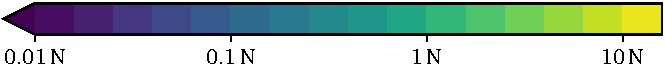
\includegraphics{biomech2ErrorForce_7}%
  \\[2mm]%
  \subcaptionbox{%
    $\abs{\forceXref - \forceXintp[p]}$ for
    $X = \mathrm{T}$ \emph{(left)} and
    $X = \mathrm{B}$ \emph{(right).}%
  }[74mm]{%
    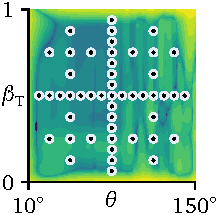
\includegraphics{biomech2ErrorForce_1}%
    \hfill%
    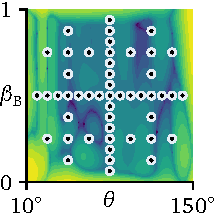
\includegraphics{biomech2ErrorForce_2}%
  }%
  \hfill%
  \subcaptionbox{%
    $\abs{\forceXref - \forceXintp[p,\cc]}$ for
    $X = \mathrm{T}$ \emph{(left)} and
    $X = \mathrm{B}$ \emph{(right).}%
  }[74mm]{%
    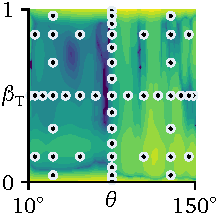
\includegraphics{biomech2ErrorForce_3}%
    \hfill%
    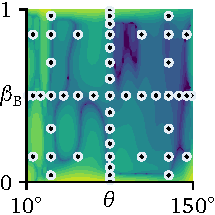
\includegraphics{biomech2ErrorForce_4}%
  }%
  \caption[Absolute error of muscle forces]{%
    Absolute error of muscle forces $\forceT, \forceB$ for
    modified cubic B-splines ($p = 3$)
    on sparse grids of uniform type \emph{(left two plots)} and
    of Clenshaw--Curtis type \emph{(right two plots)}
    together with the points of the sparse grid \emph{(dots).}%
  }%
  \label{fig:biomech2ErrorForce}%
\end{figure}

\pagebreak

\paragraph{Error of the equilibrium elbow angle}

The relative $\Ltwo$ errors
$\normLtwo{\equielbangref{\forceL} - \equielbangintp{\forceL}}/
\normLtwo{\equielbangref{\forceL}}$
of the equilibrium elbow angle function are shown in
\cref{tbl:biomech2ErrorL2_1} for the load of
$\forceL = \SI{22}{\newton}$.
Modified cubic Clenshaw--Curtis B-splines achieve the best results.
Therefore, we use this type of hierarchical basis
for the remainder of this chapter.
Pointwise plots of the absolute error
$\abs{\equielbangref{\forceL} - \equielbangintp[p,\cc]{\forceL}}$
are presented in \cref{fig:biomech2ErrorEquilibriumAngle}.
Again, the maximal error is comparatively small:
For $\forceL = \SI{22}{\newton}$, it is only \ang{0.886}.
If we restrict the domain to $\clint{0.15, 0.85}^2$,
then this maximal error drops to \ang{0.103} (or \ang{;6.18;}),
as the areas near the boundary of $\clint{\*0, \*1}$
contribute the most to the error.

\begin{figure}
  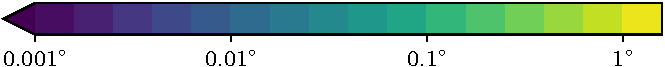
\includegraphics{biomech2ErrorEquilibriumAngle_5}%
  \\[2mm]%
  \subcaptionbox{%
    $\forceL = \SI{22}{\newton}$%
  }[49mm]{%
    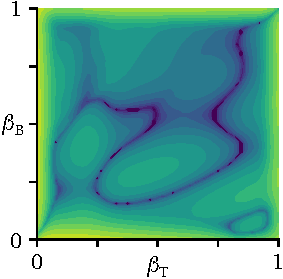
\includegraphics{biomech2ErrorEquilibriumAngle_1}%
  }%
  \hfill%
  \subcaptionbox{%
    $\forceL = \SI{-60}{\newton}$%
  }[49mm]{%
    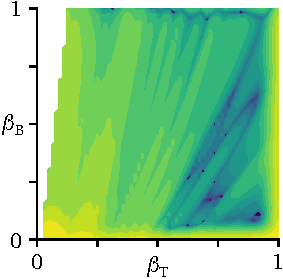
\includegraphics{biomech2ErrorEquilibriumAngle_2}%
  }%
  \hfill%
  \subcaptionbox{%
    $\forceL = \SI{180}{\newton}$%
  }[49mm]{%
    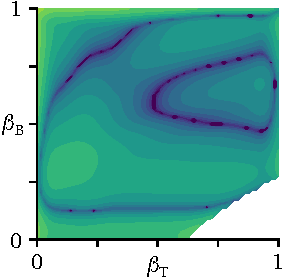
\includegraphics{biomech2ErrorEquilibriumAngle_3}%
  }%
  \caption[Absolute error of the equilibrium elbow angle]{%
    Absolute error
    $\abs{\equielbangref{\forceL} - \equielbangintp[p,\cc]{\forceL}}$
    of the equilibrium elbow angle for
    modified hierarchical cubic Clenshaw--Curtis B-splines ($p = 3$)
    for different loads $\forceL$.
    In the empty areas, at least one of
    $\equielbangref{\forceL}$ and $\equielbangintp[p,\cc]{\forceL}$
    is not well-defined (see \cref{eq:equilibriumAngle}).%
  }%
  \label{fig:biomech2ErrorEquilibriumAngle}%
\end{figure}



\subsection{Test Scenario}
\label{sec:734scenario}

\paragraph{Definition of the test scenario}

In the following, we want to assess the performance
of the sparse grid interpolants for the optimization problems
\ref{item:biomech2MinSum} and \ref{item:biomech2MinDist}.
For this goal, we create a test scenario \cite{Valentin18Gradient}
that simulates a pseudo-dynamic sequence of motions
by varying the load force and/or the target elbow angle
in discrete time steps $t$ as seen in \cref{fig:biomech2ScenarioA_1}.
The test scenario is as follows:
%
\begin{figure}
  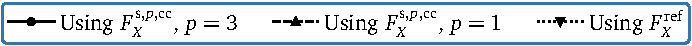
\includegraphics{biomech2ScenarioA_5}%
  \\[2mm]%
  \subcaptionbox{%
    Load $\forceL$ and target elbow angle $\tarelbang$.%
    \label{fig:biomech2ScenarioA_1}%
  }[73.3mm]{%
    \hspace*{4.5mm}%
    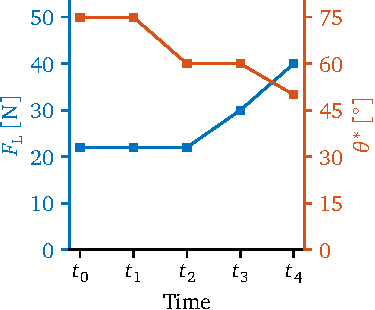
\includegraphics{biomech2ScenarioA_1}%
    \hspace*{2.4mm}%
  }%
  \hfill%
  \subcaptionbox{%
    Optimal activation parameters $\actT$ and $\actB$.%
    \label{fig:biomech2ScenarioA_2}%
  }[73.3mm]{%
    \hspace*{0.0mm}%
    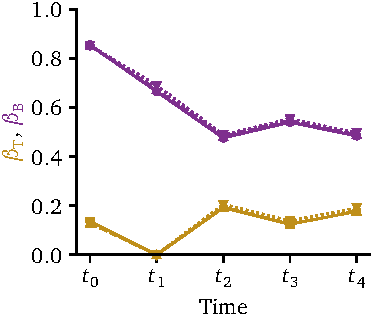
\includegraphics{biomech2ScenarioA_2}%
    \hspace*{9.8mm}%
  }%
  \\[1mm]%
  \subcaptionbox{%
    Deviation $\abs{\equielbang{\forceL} - \tarelbang}$
    of attained elbow angle to target and
    deviation \smash{$|\momentref|$} of the moment from equilibrium.%
    \label{fig:biomech2ScenarioA_3}%
  }[73.3mm]{%
    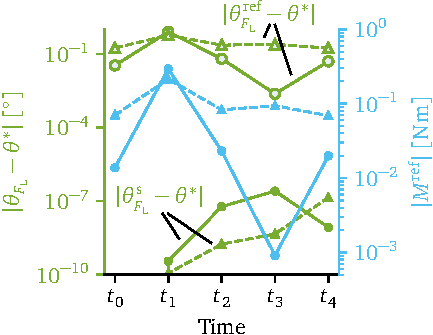
\includegraphics{biomech2ScenarioA_3}%
  }%
  \hfill%
  \subcaptionbox{%
    Number of evaluations of $\equielbang{\forceL}$
    and number of Newton iterations per evaluation
    of $\equielbang{\forceL}$.%
    \label{fig:biomech2ScenarioA_4}%
  }[73.3mm]{%
    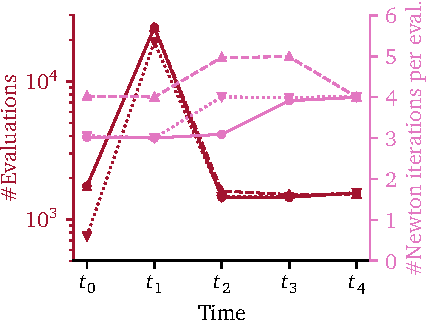
\includegraphics{biomech2ScenarioA_4}%
  }%
  \caption[Settings and results of the test scenario]{%
    Setting (a) of the test scenario and corresponding results (b, c, d).%
  }%
  \label{fig:biomech2ScenarioA}%
\end{figure}
%
\begin{enumerate}
  \item
  Find a feasible initial solution for problem \ref{item:biomech2MinSum}
  with $\forceL(t_0) \ceq \SI{22}{\newton}$ and
  $\tarelbang(t_0) \ceq \ang{75}$.
  
  \item
  Apply \ref{item:biomech2MinSum} with $\forceL(t_1) \ceq \SI{22}{\newton}$ and
  $\tarelbang(t_1) \ceq \ang{75}$.
  
  \item
  Apply \ref{item:biomech2MinDist} with $\forceL(t_2) \ceq \SI{22}{\newton}$ and
  $\tarelbang(t_2) \ceq \ang{60}$ (changed target angle).
  
  \item
  Apply \ref{item:biomech2MinDist} with $\forceL(t_3) \ceq \SI{30}{\newton}$ and
  $\tarelbang(t_3) \ceq \ang{60}$ (changed load).
  
  \item
  Apply \ref{item:biomech2MinDist} with $\forceL(t_4) \ceq \SI{40}{\newton}$ and
  $\tarelbang(t_4) \ceq \ang{50}$ (changed load and target angle).
\end{enumerate}
%
For each of the steps 2 to 5, the activation levels $\actT, \actB$ obtained
in the previous step (i.e., either the feasible initial solution
of step 1 or the optimal solution of steps 2 to 4) are used
as the input of the optimization problem
\ref{item:biomech2MinSum} or \ref{item:biomech2MinDist}.
The feasible initial solution in step 1 is determined as explained
in \cref{sec:513gradientBasedConstrained}.

\paragraph{Solutions of problem \ref{item:biomech2MinSum}}

We note that independently of $\forceL$ and $\tarelbang$,
every solution $(\actT, \actB)$ of problem \ref{item:biomech2MinSum} will be
on the boundary part of the domain $\clint{\*0, \*1}$,
on which at least one activation parameter vanishes, i.e.,
\begin{equation}
  \{(\actT, \actB) \in \clint{\*0, \*1} \mid
  (\actT = 0) \lor (\actB = 0)\}.
\end{equation}
The reason is that the two muscles triceps and biceps are antagonistic
(see \cref{sec:711models}), meaning that they work against each other.
If both $\actT > 0$ and $\actB > 0$, then the body will waste energy,
as the same target elbow angle can be attained by reducing both
$\actT$ and $\actB$ simultaneously, thus requiring less energy.
A visual example for this is \cref{fig:biomech2ReferenceEquilibriumAngle},
where the contour lines generally go from the bottom left
(small $\actT, \actB$) to the top right (large $\actT, \actB$).
This issue may be prevented by either
more complicated musculoskeletal models with more
than two muscles or different optimization problems
such as problem \ref{item:biomech2MinDist},
where the objective function differs.

\paragraph{Plots of optimization results}

\Cref{fig:biomech2ScenarioA_2,fig:biomech2ScenarioA_3,fig:biomech2ScenarioA_4}
show the results of the test scenario using the muscle forces
$\forceXintp[p,\cc]$ obtained by interpolating with
modified hierarchical cubic Clenshaw--Curtis B-splines (solid lines, $p = 3$).
As comparison, we repeat the solution process
with the forces obtained by interpolating with the
corresponding hierarchical piecewise linear basis (dashed lines, $p = 1$) and
with the reference forces $\forceXref$ (dotted lines).
For the piecewise linear basis,
we use exactly the same method as for the cubic case
(Newton method for $\equielbangintp{\forceL}$,
Augmented Lagrangian with adaptive gradient descent for the
solution of problems \ref{item:biomech2MinSum} and \ref{item:biomech2MinDist}),
although the derivatives of the muscle forces are discontinuous.
For the reference forces, we use the fact that the reference surrogates
are full grid spline interpolants, which can be explicitly differentiated.
Without the full grid interpolants,
we would have to approximate the derivatives with finite differences.

\vspace*{\fill}
\pagebreak

\paragraph{Equilibrium elbow angle}

In \cref{fig:biomech2ScenarioA_2}, we see that the activation levels
of all three methods are more or less the same.
However, \cref{fig:biomech2ScenarioA_3} reveals that even these small
differences lead to deviations of the resulting equilibrium elbow angle
to the target angle that differ by up to two orders of magnitude.
The two green lines with filled markers at the bottom of
\cref{fig:biomech2ScenarioA_3} show the error of
the equilibrium elbow angle $\equielbangintp{\forceL}$
using sparse grid interpolation to the desired target angle $\tarelbang$.
Unsurprisingly, this error is very small as
it is minimized by the optimizer as part of the constraint.
The true error, which is obtained by
using the reference equilibrium elbow angle $\equielbangref{\forceL}$,
is in general much larger
(top two green lines in \cref{fig:biomech2ScenarioA_3}
with hollow markers).
We see that the cubic B-splines decrease the error
by up to two orders of magnitude compared to the
piecewise linear basis.
There are two reasons for this:
First, the error of $\equielbang{\forceL}$ is generally smaller
when using higher-order B-splines as we have seen above.
Second, higher-order B-splines are continuously differentiable,
which makes them suitable for gradient-based optimization.
In contrast, the surrogates obtained by piecewise linear interpolation
have kinks, which may complicate finding optimal points
in the augmented Lagrangian and Newton methods.

\paragraph{Number of evaluations and Newton iterations}

This is supported by \cref{fig:biomech2ScenarioA_4},
which shows the number of evaluations of $\equielbang{\forceL}$
during the optimization and the average number of Newton iterations
per evaluation.
While the number of total evaluations is similar for all three methods,
the number of required Newton iterations to achieve convergence
is in general around \SI{50}{\percent} larger for the piecewise linear
basis functions.



\subsection{Spatial Adaptivity}
\label{sec:735adaptivity}

\paragraph{Generation of a spatially adaptive sparse grid}

As mentioned in \cite{Valentin18Gradient}, spatial adaptivity
may be employed to reduce the number of necessary muscle force samples
even further,
especially for more complicated musculoskeletal systems with
more parameters.
To verify this statement, we remove all grid points
$(\elbang^{(k,\cc)}, \actX^{(k,\cc)})$
from the regular sparse Clenshaw--Curtis grid that satisfy
\begin{equation}
  \frac{
    \abs{\alpha_\mathrm{T}^{(k,p,\cc)}}
  }{
    \max_{k'} \abs{\alpha_\mathrm{T}^{(k',p,\cc)}}
  } < \SI{1}{\percent}
  \quad\text{and}\quad
  \frac{
    \abs{\alpha_\mathrm{B}^{(k,p,\cc)}}
  }{
    \max_{k'} \abs{\alpha_\mathrm{B}^{(k',p,\cc)}}
  } < \SI{1}{\percent},
\end{equation}
where $\alpha_X^{(k,p,\cc)}$ ($X \in \{\mathrm{T}, \mathrm{B}\}$)
is the hierarchical surplus of the basis function $\bspl[\cc,\modified]{k}{p}$
corresponding to $(\elbang^{(k,\cc)}, \actX^{(k,\cc)})$.
For higher-dimensional models,
one would of course not sample muscle data on a regular sparse grid
and then coarsen the data by removing points,
but rather use an a posteriori adaptivity criterion to
decide which grid points to refine iteratively.

\paragraph{Comparison with the regular case}

For the cubic case $p = 3$,
the resulting force interpolants $\forceXintp[p,\cc,\mathrm{adap}]$ together
with the spatially adaptive sparse grid
(which has been coarsened from 49 to 28 points) and
equilibrium elbow angle $\equielbangintp[p,\cc,\mathrm{adap}]{\forceL}$
for $\forceL = \SI{22}{\newton}$ are shown in
\cref{fig:biomech2SpatiallyAdaptive}.
The sparse grid is almost dimensionally adaptive,
as $\forceXref$ seems to be almost linear in the $\actX$ direction
for both $X = \mathrm{T}$ and $X = \mathrm{B}$.
The errors increase slightly:
The relative $\Ltwo$ force errors for $(\mathrm{T}, \mathrm{B})$ increase
from $(\SI{3.31}{\permille}, \SI{3.56}{\permille})$
to $(\SI{3.36}{\permille}, \SI{4.43}{\permille})$,
and the absolute $\Linfty$ errors increase
from $(\SI{10.6}{\newton}, \SI{9.51}{\newton})$
to $(\SI{12.3}{\newton}, \SI{9.57}{\newton})$.
In addition, the relative $\Ltwo$ and absolute $\Linfty$ errors
for $\equielbang{\forceL}$ increase
from \SI{2.83}{\permille} and \ang{0.886}
to \SI{4.12}{\permille} and \ang{1.09}, respectively.
While all these errors are somewhat larger than for the regular sparse grid,
they are still at an acceptable level,
but the number of necessary muscle force evaluations is halved compared
to the regular case.
Additionally, the solution of the test scenario doesn't change significantly
due to the similar errors of $\forceX$ and $\equielbang{\forceL}$.

\begin{figure}
  \hspace*{2mm}%
  \raisebox{0.2mm}{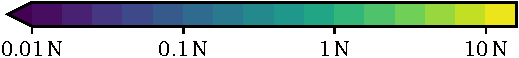
\includegraphics{biomech2ErrorForce_8}}%
  \hspace*{12mm}%
  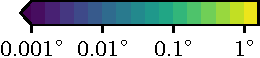
\includegraphics{biomech2ErrorEquilibriumAngle_6}%
  \\[2mm]%
  \subcaptionbox{%
    $\abs{\forceTref - \forceTintp[p,\cc,\mathrm{adap}]}$%
  }[49mm]{%
    \raisebox{1.02mm}{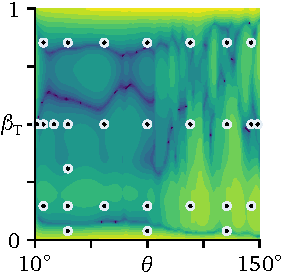
\includegraphics{biomech2ErrorForce_5}}%
  }%
  \hfill%
  \subcaptionbox{%
    $\abs{\forceBref - \forceBintp[p,\cc,\mathrm{adap}]}$%
  }[49mm]{%
    \raisebox{1.02mm}{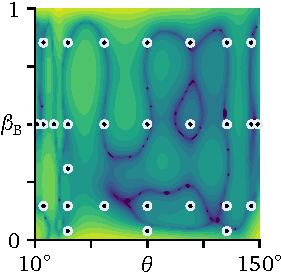
\includegraphics{biomech2ErrorForce_6}}%
  }%
  \hfill%
  \subcaptionbox{%
    $\abs{
      \equielbangref{\forceL} - \equielbangintp[p,\cc,\mathrm{adap}]{\forceL}
    }$
    for $\forceL = \SI{22}{\newton}$%
  }[49mm]{%
    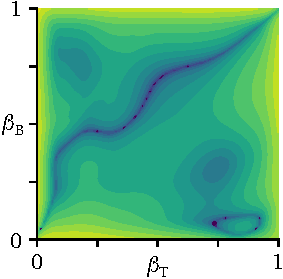
\includegraphics{biomech2ErrorEquilibriumAngle_4}%
  }%
  \caption[%
    Errors of muscle forces and equilibrium angle
    for the spatially adaptive case%
  ]{%
    Errors of muscle forces and equilibrium elbow angle
    for the spatially adaptive case
    (modified hierarchical cubic Clenshaw--Curtis B-splines,
    i.e., $p = 3$) together with the points of the
    spatially adaptive sparse grid \emph{(dots).}%
  }%
  \label{fig:biomech2SpatiallyAdaptive}%
\end{figure}


\cleardoublepage
